\begin{figure}[h!]
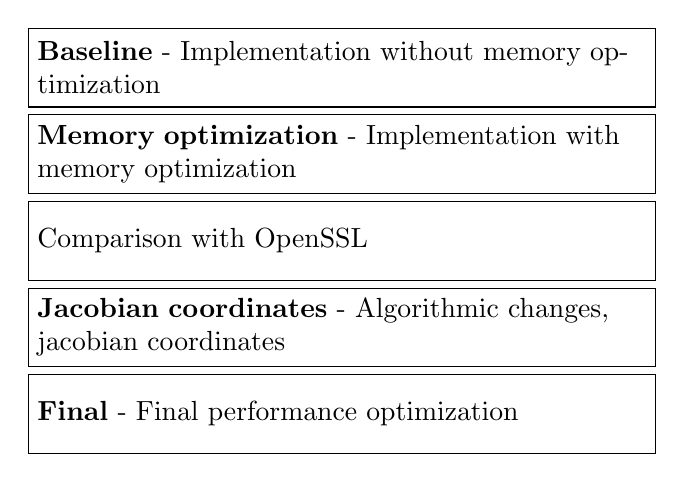
\begin{tikzpicture}[
rect/.style={
draw,
text width=22em,
minimum height = 1cm
},node distance=1.1cm
]
\node[rect] (1) {\textbf{Baseline} - Implementation without memory optimization};
\node[rect, below of=1] (2) {\textbf{Memory optimization} - Implementation with memory optimization};
\node[rect, below of=2] (3) {Comparison with OpenSSL};
\node[rect, below of=3] (4) {\textbf{Jacobian coordinates} - Algorithmic changes, jacobian coordinates};
\node[rect, below of=4] (5) {\textbf{Final} - Final performance optimization };

\end{tikzpicture}
\caption{approach\label{fig:method}}
\end{figure}

\mypar{Baseline} 
Some information about the first baseline

\mypar{Memory optimization}

\mypar{First comparision with OpenSSL}
Realization that the chosen algorithm is not optimal.

\mypar{Jacobian coordinates}
Introduction of the Jacobian coordinates
Precomputation of the Points

\mypar{Final}
Final optimizations like function stitching and inline assembly 

Now comes the ``beef'' of the paper, where you explain what you
did. Again, organize it in paragraphs with titles. As in every section
you start with a very brief overview of the section.

For this class, explain all the optimizations you performed. This mean, you first very briefly
explain the baseline implementation, then go through locality and other optimizations, and finally SSE (every project will be slightly different of course). Show or mention relevant analysis or assumptions. A few examples: 1) Profiling may lead you to optimize one part first; 2) bandwidth plus data transfer analysis may show that it is memory bound; 3) it may be too hard to implement the algorithm in full generality: make assumptions and state them (e.g., we assume $n$ is divisible by 4; or, we consider only one type of input image); 4) explain how certain data accesses have poor locality. Generally, any type of analysis adds value to your work.

As important as the final results is to show that you took a structured, organized approach to the optimization and that you explain why you did what you did.

Mention and cite any external resources including library or other code.

Good visuals or even brief code snippets to illustrate what you did are good. Pasting large amounts of code to fill the space is not good.